% +------------------------------------------------------------------------+
% | CGAL Reference Manual:  snapRounding.tex
% +------------------------------------------------------------------------+
% | snap rounding of line segments
% |
% | 9.4.00   Eli Packer
% | 
%\RCSdef{\largestEmptyRectangleRev}{$Revision$}
%\RCSdefDate{largestEmptyRectangleDate}{$Date$}
% +------------------------------------------------------------------------+

\ccParDims

% \usepackage{graphics, amssymb,epsfig}

\chapter{Largest Empty Rectangle}
\label{chapterLer}
%\ccChapterRelease{\largestEmptyRectangleRev. \ \largestEmptyRectangleDate}\\
\ccChapterAuthor{Eli Packer}

% +------------------------------------------------------------------------+
\section{Overview}
The Largest Empty Rectangle problem answers the following query. Given
a set of points in the plane and a bounding box( iso-rectangle) that bounds them,
find the iso-rectangle with the largest area among all iso-rectangles that are
inside the above bounding box and do not contain any point of the point set.
See Figure~\ref{fig:ler1} for an illustration.

\begin{figure}[h]
\begin{ccTexOnly}
    \centerline{
      \includegraphics{ler_example.ps}
    }
\end{ccTexOnly}

\caption{An example of the largest empty iso rectangle of a set of points
\label{fig:ler1}}

\begin{ccHtmlOnly}
    <P>
    <center>
        <img src="ler_example.gif"  border=0 alt="example output">
        <!--An example of the largest empty iso rectangle of a set of points-->
    </center>
\end{ccHtmlOnly}
\end{figure}

The algorithm is an implementation of \cite{o-naler-90}. The runtime of an
insertion or a removal is $O(\log n)$. A query takes $O(n^2)$ worst
case time and $O(n \log n)$ expected time. The working storage is $
O(n)$.


% +========================================================================+
\section{Examples of Largest Empty Rectangle}
% +========================================================================+

The following example generates the Largest Empty Rectangle of a set
of points.

\ccIncludeExampleCode{../../examples/Largest_empty_rect_2/example.C}

% +--------------------------------------------------------+

% EOF


